% !TeX root = ./maltoni_niccolo_tesi.tex
% !TeX encoding = UTF-8 Unicode
% !TeX spellcheck = it_IT
% !TeX program = arara
% !TeX options = --log --verbose --language=it "%DOC%"

% arara: lualatex:      { interaction: batchmode, shell: yes }
% arara: frontespizio:  { interaction: batchmode, engine: lualatex, shell: yes }
% arara: biber
% arara: lualatex:      { interaction: batchmode, shell: yes }
% arara: lualatex:      { interaction: nonstopmode, shell: yes, synctex: yes }

\documentclass[%
  a4paper,                % formato di pagina A4
  fontsize=12pt,          % corpo del testo a 12pt
  % la dimensione 12pt automaticamente imposta \footnotesize a 10pt
  twoside,                % (oneside|twoside) documento a singola o doppia facciata,
  openright,              % (openany|openright) fa cominciare un capitolo nella successiva pagina a disposizione o sempre in una pagina destra
  % twocolumn,            % dà a LaTeX le istruzioni per comporre l'intero documento su due colonne
  titlepage,              % (titlepage|notitlepage) se dopo il titolo del documento debbaavere  inizio  una  nuova  pagina
  % fleqn,                % allinea le formule a sinistra rispetto a un margine rientrato
  % leqno,                % mette la numerazione delle formule a sinistra anziché a destra
  final                   % (draft|final) scelta tra bozza o finale, influenza il comportamento degli altri pacchetti
  headings=standardclasses, % changes the font of all section heading levels to serif
  headings=big,             % revert to default heading size that headings=standardclasses changes
  chapterprefix=false       % reverse the chapterprefix=true option that headings=standardclasses sets
]{scrbook}

\usepackage{fancyvrb}       % fornisce l'ambiente VerbatimOut e modifica listati di codice

\begin{VerbatimOut}{\jobname.xmpdata}
\Title{Progettazione di un sistema web per la simulazione di programmi aggregati}
\Author{Niccolò Maltoni}
\Copyright{Questo documento è fornito sotto licenza Creative Commons Attribution-ShareAlike 4.0 International}
\CopyrightURL{http://creativecommons.org/licenses/by-sa/4.0}
\end{VerbatimOut}

\usepackage{unibotesi}
\def\blx@nowarnpolyglossia{}
\usepackage[automark,headsepline]{scrlayer-scrpage}
\clearpairofpagestyles{}
\cfoot[\pagemark]{\pagemark}
\lehead{\headmark}
\rohead{\headmark}
\pagestyle{scrheadings}

\begin{document}

  \frontmatter{}

  \begin{Preambolo*}
  \usepackage{fontspec}
  \defaultfontfeatures{ Scale = MatchUppercase }
  \setmainfont{libertinusserif}[
    Scale=1.0,
    Ligatures={Common, TeX},
    % Numbers={OldStyle, Proportional},
    UprightFont={*-regular},
    BoldFont={*-bold},
    ItalicFont={*-italic},
    BoldItalicFont={*-bolditalic},
    Extension=.otf
  ]
  \setsansfont{libertinussans}[
    Ligatures={Common, TeX},
    % Numbers={OldStyle, Proportional},
    UprightFont={*-regular},
    BoldFont={*-bold},
    ItalicFont={*-italic},
    % BoldItalicFont={*-bolditalic},
    Extension=.otf
  ]
  \setmonofont{libertinusmono}[
    Scale=0.95,
    UprightFont={*-regular},
    % BoldFont={*-bold},
    % ItalicFont={*-italic},
    % BoldItalicFont={*-bolditalic},
    Extension=.otf
  ]
\end{Preambolo*}
\begin{frontespizio}
  \Universita{Bologna}        % aggiunge da sé “Università degli Studi di”.
  \Istituzione{%
    Alma Mater Studiorum --- Università di Bologna \\%
    Campus di Cesena%
  }
  \Divisione{Dipartimento di Informatica --- Scienza e Ingegneria}
  \Corso[Laurea magistrale]{Ingegneria e Scienze Informatiche}
  \Annoaccademico{2019--2020}
  \Titolo{Progettazione di una piattaforma web\\per la simulazione di programmi aggregati}
  \Sottotitolo{Tesi in Pervasive Computing}
  % \Preambolo{\renewcommand{\frontsmallfont}[1]{\small}}       % non viene stampata la matricola
  % \Preambolo{\renewcommand{\frontsmallfont}[1]{\small Matr.}} % abbrevia la matricola
  \Candidato[840825]{Niccolò~Maltoni}
  \NCandidato{Presentata da}  % sostituisce la parola “Candidato”
  \Relatore{Prof.~Mirko~Viroli}
  \Correlatore{Prof.~Danilo~Pianini}
  \Piede{%                    % sostituisce la scritta “Anno Accademico” nel piede
    III sessione di laurea \\%
    Anno Accademico 2019--2020%
  }
\end{frontespizio}

% Necessario per Overleaf: compila il TeX del frontespizio subito dopo averlo generato
\IfFileExists{\jobname-frn.pdf}{}{%
\immediate\write18{lualatex \jobname-frn}}

  \clearemptydoublepage{}
\thispagestyle{empty}
\vspace*{20ex}
\begin{flushright}
    \begin{LARGE}
        \textbf{Parole chiave}\\
        \vspace{5ex}
    \end{LARGE}
    \begin{normalsize}
        \textbf{%
            Aggregate programming\\%
            \medskip
            Protelis%
            \medskip
            Applicazione web
        }
    \end{normalsize}
\end{flushright}
\vfill

  \clearemptydoublepage{}
\thispagestyle{plain}
\null{}\vspace{\stretch{1}}
\begin{flushright}
    \textit{Dedica}
\end{flushright}
\vspace{\stretch{2}}\null{}

  \begin{abstract}
  \strong{TODO}
  \emph{\lipsum[1-2]} % ChkTeX 8
\end{abstract}


  \tableofcontents

  \mainmatter{}

  \addchap{Introduzione}

  \part{Background}
    \chapter{Motivazioni}\label{ch:motivations}


  \section{Stato dell'arte}

  \section{Prospettive}

  \section{Dettaglio del problema e approccio}


    \chapter{Programmazione aggregata}

La crescita esponenziale di dispositivi informatici di varia natura inseriti in contesti quotidiani ha avuto un impatto globale notevole.
Questo insieme di entità connesse (\Cref{fig:iot}) ha dato luogo a ciò che viene definito \emph{Internet of Things} (\emph{IoT}).

\begin{figure}
  \centering
  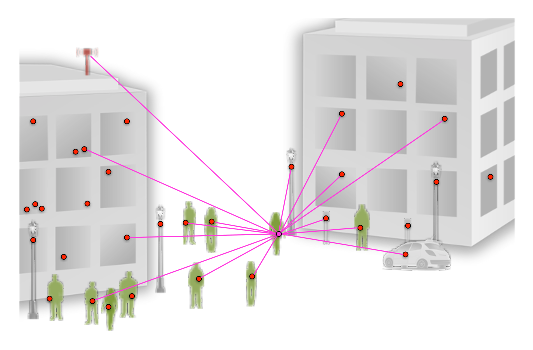
\includegraphics[width=0.8\textwidth]{res/fig/iot.eps}%
  \caption{Possibile scenario di rete in contesto urbano~\cite{7274429}}%
  \label{fig:iot}
\end{figure}

L'approccio iniziale per la realizzazione di sistemi in questo contesto è stato incentrato sui classici paradigmi ``\emph{single device view point}'',
i quali vedono al centro dell'attenzione il singolo dispositivo e le interazioni che questo ha con gli altri e con l'ambiente.
Tale approccio si è ben presto rivelato inadeguato % TODO: perché?

    \chapter{Progettazione di sistemi web}\label{chap:web}
  Il World Wide Web ha assunto un ruolo sempre più centrale nella quotidianità delle persone e nelle dinamiche di business.
  In particolare, il modello di comunicazione è sempre più virato verso scenari distribuiti,
  nei quali piattaforme eterogenee riescono a comunicare tra loro condividendo informazioni di diverso tipo attraverso la rete internet.

  Anche i pattern di progettazione e le tecnologie implementative sono cresciute altrettanto velocemente negli ultimi anni, cambiando anche radicalmente gli approcci di interazione possibili.
  Risulta dunque importante prestare attenzione allo stato dell'arte in tal senso, chiarendo quali siano i pattern più adatti e moderni per il contesto d'uso di questa tesi.

  \section{Architetture, framework e stack}\label{sec:web-architecture}

  Con \emph{sistema web} si intende genericamente un sistema software distribuito che coinvolge una o più entità server che espongono in rete API di varia natura, con le quali entità client possono comunicare per usufruire dei servizi.
  Generalmente, in contesto web i client sono costituiti da pagine web aperte nei browser degli utenti.

  Le possibilità di progettazione di un'applicazione web possono essere molto differenti e nel tempo si è vista una vera e propria evoluzione in tal senso:

  \begin{enumerate}
    \item
      nel periodo iniziale del web, ciascuna pagina web era inviata al client come un documento statico;
      l'interazione dell'utente con il sistema avveniva attraverso la navigazione, che comportava l'apertura di una sequenza di pagine a seconda delle esigenze.
      Questo tipo di interazione era però lenta, in quanto coinvolgeva sempre la ricezione di una nuova pagina dal server.
    \item
      successivamente, nel 1995, con l'introduzione da parte di NetScape di JavaScript (di cui tratteremo meglio nella~\Cref{subsec:js}) come linguaggio di scripting client-side, i programmatori hanno avuto la possibilità di inserire elementi dinamici nelle pagine web.
      In questo modo, era possibile effettuare alcune operazioni anche localmente, riducendo di fatto il numero di pagine intere scambiate con il server.
    \item
      un'ulteriore innovazione apparve l'anno seguente, quando Macromedia introdusse \emph{Flash}:
      esso era un plugin per i browser che permetteva di riprodurre animazioni vettoriali e gestire le interazioni con l'utente, in modo simile a quanto fatto da JavaScript.
    \item
      il termine ``\emph{web application}'' nasce però con l'introduzione della versione 2.2 della Java Servlet Specification~\cite{java1999specification} nel 1999.
      anche in questo caso, però, il server ha un ruolo centrale e ancora il concetto di \emph{ajax} (\emph{Asynchronous JavaScript + XML}) non è stato introdotto.
    \item
      successivamente vi sono stati diversi miglioramenti incrementali, fino ad arrivare allo standard HTML5~\cite{Smith2008}:
      con quest'ultimo, infatti, introduce il supporto nativo ai contenuti multimediali ed arricchisce la semantica del documento, oltre a migliorare l'integrazione con JS\@.
      Con questo standard, diventa sempre più comune il concetto di \emph{Single-page application} (SPA), secondo il quale la pagina viene caricata una sola volta, e poi modificata dinamicamente tramite chiamate specifiche al server.
      Nascono numerosi framework client-side (come Angular, Ember o React) e l'impiego del server viene sempre più circoscritto al fornire API per accesso controllato ai dati (ad esempio, un database) o per computazioni complesse.
  \end{enumerate}

  % TODO: Service-Oriented Architecture e Resource-Oriented architecture

  \section{Linguaggi ad uso web}\label{sec:lang}
    In questa \nameCref{sec:lang} verranno analizzati i principali linguaggi di programmazione utilizzati recentemente per lo sviluppo della componente frontend delle applicazioni web.
    In particolare, verranno presi in considerazione i due linguaggi più popolari, ossia \emph{JavaScript} e il suo superset \emph{TypeScript}, e due linguaggi di nicchia che offrono una valida alternativa: \emph{Scala.js} e \emph{Kotlin/JS}\@.

    \subsection{JavaScript e ECMAScript}\label{subsec:js}

    \emph{JavaScript} è un linguaggio di scripting debolmente tipizzato orientato agli oggetti, agli eventi e alle funzioni.
    Sviluppato originariamente nel 1995 da Brendan Eich della Netscape Communications (inizialmente con il nome di \emph{Mocha} e poi \emph{LiveScript}),
    esso è stato concepito con lo scopo di avere un linguaggio di scripting per il browser Netscape Navigator più semplice da apprendere rispetto a quelli esistenti.
    JavaScript è stato standardizzato per la prima volta nel 1997 dalla ECMA con il nome di \emph{ECMAScript}~\cite{ECMA-262,ISO:1998} e l'attuale versione è la decima.

    Il linguaggio è attualmente il più popolare per uso web, in quanto l'unico ad essere supportato da tutti i browser moderni, almeno nelle sue feature principali.
    Diversi linguaggi, come quelli che vedremo in seguito, vengono transpilati in una versione sufficientemente supportata di JS per poter essere eseguiti nei browser.

    Analizzato dal punto di vista tecnico, esso presenta i seguenti aspetti strutturali:

    \begin{description}
      \item[Imperativo e strutturato]
        Il linguaggio si presenta con una sintassi di programmazione strutturata standard, con il supporto a tutte le strutture di controllo tradizionali.
        Una parziale differenza era nella gestione della visibilità delle variabili (\emph{scope}):
        inizialmente, JavaScript garantiva solo la visibilità a livello di funzione (\emph{function scope}) tramite la parola chiave \texttt{var};
        con ECMAScript 6 è stato aggiunto il supporto alla visibilità a livello di blocco (\emph{block scope}).

      \item[Tipizzazione dinamica]
        % https://developer.mozilla.org/en-US/docs/Web/JavaScript/Data_structures
        JavaScript è un linguaggio debolmente tipizzato:
        alle variabili non sono associati dei tipi di dato, ma solo dei valori, che possono dinamicamente cambiare tipo durante il ciclo di vita della variabile.
        La tipizzazione dinamica consente lo stile di tipizzazione chiamato \emph{Duck Typing}~\cite{10.1145/2103621.2103686}:
        è possibile determinare la semantica di un oggetto in base ai metodi ed alle proprietà che esso possiede,  non in base al suo tipo.

      \item[Orientamento agli oggetti Prototype-based]
        A differenza di altri linguaggi orientato agli oggetti (come Java o C++), JavaScript non fornisce un'implementazione del concetto di \emph{classe}~\cite{Ungar1991}:
        la stessa keyword \texttt{class}, introdotta con ES6, non è altro che zucchero sintattico per migliorare l'interazione da parte dei nuovi sviluppatori con il prototipo.

        In termini di ereditarietà, infatti, JS prevede un solo costrutto: gli \emph{oggetti}.
        Ogni oggetto ha un collegamento interno ad un altro oggetto chiamato \emph{prototype}.
        Questo oggetto prototipo ha a sua volta un suo prototype, e così via finché si raggiunge un oggetto con la proprietà prototipo settata a \texttt{null}.
        \texttt{null}, per definizione, non ha un prototype ed agisce come link finale nella \emph{catena di prototipi}.

        Quasi tutti gli oggetti in JavaScript sono istanze di \texttt{Object}, che risiede in cima alla catena dei prototipi.
        % In JavaScript, è possibile aggiungere proprietà a qualsiasi oggetto in fase di esecuzione.

      \item[First-class function]
        JavaScript offre un supporto di prima classe alle funzioni, che sono considerate oggetti;
        come tali, esse possono avere delle proprietà, come ad esempio \texttt{.bind()} e \texttt{.call()}. % ChkTeX 36

        Ciascuna funzione costituisce una chiusura lessicale.

        All'interno di oggetti, proprietà di tipo funzione vengono utilizzate come costruttori e come metodi.
        Infine, le funzioni possono essere utilizzati per l'implementazione di \emph{pattern di ruolo} come i \emph{tratti} e i \emph{mixin}.

      \item[Web APIs]
        Con ECMAScript si standardizza la componente \emph{core} del linguaggio, che può eseguire in ambienti browser come su interpreti non legati strettamente al web (come ad esempio Node.js~\cite{5617064}).
        Ciascuno degli ambienti nei quali il linguaggio viene interpretato mettono a disposizione delle API specifiche per l'interazione con la piattaforma;
        quando si fa riferimento al browser, tali supporti sono chiamati \emph{Web APIs}.

        Attraverso di esse, lo sviluppatore può avere accesso agli elementi del DOM (Document Object Model) di HTML, potendo manipolare la pagina visualizzata e reagire ad eventi su di essa.

      \item[Asincronismo]
        JavaScript supporta inoltre nativamente l'esecuzione di operazioni in modo asincrono tramite il costrutto della \emph{promise}, implementato da un oggetto built-in \texttt{Promise},
        che costituisce un \emph{proxy} per un valore non necessariamente noto quando la promise viene creata.
        È poi possibile gestire il valore ottenuto con costrutti ``\emph{thenable}'' o con il \emph{pattern async/await}.
    \end{description}

    \subsection{TypeScript}\label{subsec:ts}
    TypeScript è un linguaggio di programmazione open-source sviluppato da Microsoft.
    Esso è un super-set sintatticamente rigoroso di JavaScript ES6, che si pone come obiettivo % TODO


    % \item[Operatore di coalescenza dei null e safe navigation]
    % Tradizionalmente, in JavaScript sono considerati \emph{falsy} diversi valori (come \texttt{NaN}, \texttt{0} e la stringa vuota) che non sono \texttt{null} o \texttt{undefined}
    % ma vengono trattati come valori ``non presenti'' e dunque come \texttt{false} dagli operatori booleani.
    % Sono dunque stati introdotti gli operatori di \emph{nullish coalescing} (\texttt{??}) e di \emph{safe navigation} (\texttt{.?}) per aggirare questo tipo di problema.

    \subsection{Scala.js}
    \subsection{Kotlin/Multiplatform e Kotlin/JS}


  \part{Contributo: Protelis on Web}
    \chapter{Analisi dei requisiti}
      \section{Requisiti funzionali}
      \section{Requisiti non funzionali}
    \chapter{Progettazione}
      \section{Design dell'architettura}
      \section{Mockup dell'interfaccia}
    \chapter{Implementazione}
    % \chapter{Testing}

  \part{Conclusioni}
    \chapter{Valutazione dei risultati}
    \chapter{Lavori futuri}
    \chapter{Considerazioni finali}

  \appendix
  \addpart*{\appendixname}
% \renewcommand{\thesection}{\Alph{section}}
% \renewcommand{\thesubsection}{A.\arabic{subsection}}

% \addcontentsline{toc}{section}{\appendixname}
% \addchap{\appendixname}
% \chapter*[]{\appendixname}

\begin{appendices}
  % \section{Dockerfile del server}\label{app:docker}
  \chapter{Dockerfile del server}\label{app:docker}
    \inputminted{dockerfile}{res/code/Dockerfile}
\end{appendices}


  \backmatter{}
  \nocite{7274429,PianiniSASOTutorial2017}
\printbibliography[heading=bibintoc]

  \addchap{Ringraziamenti}

% 1
% Ringrazio il professor Mirko Viroli e il professor Danilo Pianini per la bella
% opportunità che mi hanno offerto, per tutto l’aiuto datomi per realizzare
% questo progetto e per i consigli ricevuti. Ringrazio anche gli amici che mi
% sono stati accanto durante questi mesi, ma soprattutto un particolare grazie
% ai miei genitori che mi sostengono da sempre.

% 2
% Un sincero ringraziamento va a tutti coloro che mi hanno aiutato in vario modo a
% raggiungere questo traguardo. Ringrazio il professor Mirko Viroli e il professor Danilo
% Pianini per l’aiuto datomi nella realizzazione di questo progetto, sia durante l’attività
% sperimentale che per la stesura dell’elaborato finale. Ringrazio anche gli amici che ho
% avuto vicino in questi mesi, ma soprattutto un particolare grazie ai miei familiari che mi
% sostengono da sempre.


\end{document}
